\begin{aosachapter}{A 3D Modeller}{s:modeller}{Erick Dransch}

\aosasecti{Introduction}\label{introduction}

Humans are innately creative. We continuously design and build novel,
useful, and interesting things. In modern times, we write software to
assist in the design and creation process. Computer-aided design (CAD)
software allows creators to design buildings, bridges, video game art,
film monsters, 3D printable objects, and many other things on a computer
before building a physical version of the design.

At their core, CAD tools are a method of abstracting the 3-dimensional
design into something that can be viewed and edited on a 2-dimensional
screen. To fulfill that definition, CAD tools must offer three basic
pieces of functionality. Firstly, they must have a data structure to
represent the object that's being designed: this is the computer's
understanding of the 3-dimensional world that the user is building.
Secondly, the CAD tool must offer some way to display the design on the
user's screen. The user is designing a physical object with 3
dimensions, but the computer screen has only 2 dimensions. The CAD tool
must model how we perceive objects, and draw them to the screen in a way
that the user can understand all 3 dimensions of the object. Thirdly,
the CAD tool must offer a way to interact with the object being
designed. The user must be able to add to and modify the design in order
to produce the desired result. Additionally, all tools would need a way
to save and load designs from disk so that users can collaborate, share,
and save their work.

A domain-specific CAD tool offers many additional features for the
specific requirements of the domain. For example, an architecture CAD
tool would offer physics simulations to test weather and climate
stresses on the building, a 3D printing tool would have features that
check whether the object is actually valid to print, an electrical CAD
tool would simulate the physics of electricity running through copper,
and a film special effects suite would include features to accurately
simulate pyrokinetics.

However, all CAD tools must include at least the three features
discussed above: a data structure to represent the design, the ability
to display it to the screen, and a method to interact with the design.

With that in mind, let's explore how we can represent a 3D design,
display it to the screen, and interact with it, in 500 lines of Python.

\aosasecti{Rendering as a Guide}\label{rendering-as-a-guide}

The driving force behind many of the design decisions in a 3D modeller
is the rendering process. We want to be able to store and render complex
objects in our design, but we want to keep the complexity of the
rendering code low. Let us examine the rendering process, and explore
the data structure for the design that allows us to store and draw
arbitarily complex objects with simple rendering logic.

\aosasectii{Managing Interfaces and the Main
Loop}\label{managing-interfaces-and-the-main-loop}

Before we begin rendering, there are a few things we need to set up.
First, we need to create a window to display our design in. Secondly, we
want to communicate with graphics drivers to render to the screen. We
would rather not communicate directly with graphics drivers, so we use a
cross-platform abstraction layer called OpenGL, and a library called
GLUT (the OpenGL Utility Toolkit) to manage our window.

\aosasectiii{A Note About OpenGL}\label{a-note-about-opengl}

OpenGL is a graphical application programming interface for
cross-platform development. It's the standard API for developing
graphics applications across platforms. OpenGL has two major variants:
Legacy OpenGL and Modern OpenGL.

Rendering in OpenGL is based on polygons defined by vertices and
normals. For example, to render one side of a cube, we specify the 4
vertices and the normal of the side.

Legacy OpenGL provides a ``fixed function pipeline''. By setting global
variables, the programmer can enable and disable automated
implementations of features such as lighting, coloring, face culling,
etc. OpenGL then automatically renders the scene with the enabled
functionality. This functionality is deprecated.

Modern OpenGL, on the other hand, features a programmable rendering
pipeline where the programmer writes small programs called ``shaders''
that run on dedicated graphics hardware (GPUs). The programmable
pipeline of Modern OpenGL has replaced Legacy OpenGL.

In this project, despite the fact that it is deprecated, we use Legacy
OpenGL. The fixed functionality provided by Legacy OpenGL is very useful
for keeping code size small. It reduces the amount of linear algebra
knowledge required, and it simplifies the code we will write.

\aosasectiii{About GLUT}\label{about-glut}

GLUT, which is bundled with OpenGL, allows us to create operating system
windows and to register user interface callbacks. This basic
functionality is sufficient for our purposes. If we wanted a more
full-featured library for window management and user interaction, we
would consider using a full windowing toolkit like GTK or Qt.

\aosasectiii{The Viewer}\label{the-viewer}

To manage the setting up of GLUT and OpenGL, and to drive the rest of
the modeller, we create a class called \texttt{Viewer}. We use a single
\texttt{Viewer} instance, which manages window creation and rendering,
and contains the main loop for our program. In the initialization
process for \texttt{Viewer}, we create the GUI window and initialize
OpenGL.

The function \texttt{init\_interface} creates the window that the
modeller will be rendered into and specifies the function to be called
when the design needs to rendered. The \texttt{init\_opengl} function
sets up the OpenGL state needed for the project. It sets the matrices,
enables backface culling, registers a light to illuminate the scene, and
tells OpenGL that we would like objects to be colored. The
\texttt{init\_scene} function creates the \texttt{Scene} objects and
places some initial nodes to get the user started. We will see more
about the \texttt{Scene} data structure shortly. Finally,
\texttt{init\_interaction} registers callbacks for user interaction, as
we'll discuss later.

After initializing \texttt{Viewer}, we call \texttt{glutMainLoop} to
transfer program execution to GLUT. This function never returns. The
callbacks we have registered on GLUT events will be called when those
events occur.

\begin{verbatim}
class Viewer(object):
    def __init__(self):
        """ Initialize the viewer. """
        self.init_interface()
        self.init_opengl()
        self.init_scene()
        self.init_interaction()
        init_primitives()

    def init_interface(self):
        """ initialize the window and register the render function """
        glutInit()
        glutInitWindowSize(640, 480)
        glutCreateWindow("3D Modeller")
        glutInitDisplayMode(GLUT_SINGLE | GLUT_RGB)
        glutDisplayFunc(self.render)

    def init_opengl(self):
        """ initialize the opengl settings to render the scene """
        self.inverseModelView = numpy.identity(4)
        self.modelView = numpy.identity(4)

        glEnable(GL_CULL_FACE)
        glCullFace(GL_BACK)
        glEnable(GL_DEPTH_TEST)
        glDepthFunc(GL_LESS)

        glEnable(GL_LIGHT0)
        glLightfv(GL_LIGHT0, GL_POSITION, GLfloat_4(0, 0, 1, 0))
        glLightfv(GL_LIGHT0, GL_SPOT_DIRECTION, GLfloat_3(0, 0, -1))

        glColorMaterial(GL_FRONT_AND_BACK, GL_AMBIENT_AND_DIFFUSE)
        glEnable(GL_COLOR_MATERIAL)
        glClearColor(0.4, 0.4, 0.4, 0.0)

    def init_scene(self):
        """ initialize the scene object and initial scene """
        self.scene = Scene()
        self.create_sample_scene()

    def create_sample_scene(self):
        cube_node = Cube()
        cube_node.translate(2, 0, 2)
        cube_node.color_index = 2
        self.scene.add_node(cube_node)

        sphere_node = Sphere()
        sphere_node.translate(-2, 0, 2)
        sphere_node.color_index = 3
        self.scene.add_node(sphere_node)

        hierarchical_node = SnowFigure()
        hierarchical_node.translate(-2, 0, -2)
        self.scene.add_node(hierarchical_node)

    def init_interaction(self):
        """ init user interaction and callbacks """
        self.interaction = Interaction()
        self.interaction.register_callback('pick', self.pick)
        self.interaction.register_callback('move', self.move)
        self.interaction.register_callback('place', self.place)
        self.interaction.register_callback('rotate_color', self.rotate_color)
        self.interaction.register_callback('scale', self.scale)

    def main_loop(self):
        glutMainLoop()

if __name__ == "__main__":
    viewer = Viewer()
    viewer.main_loop()
\end{verbatim}

Before we dive into the \texttt{render} function, we should discuss a
little bit of linear algebra.

\aosasectii{Coordinate Space}\label{coordinate-space}

For our purposes, a Coordinate Space is an origin point and a set of 3
basis vectors, usually the $x$, $y$, and $z$ axes.

\aosasectii{Point}\label{point}

Any point in 3 dimensions can be represented as an offset in the $x$,
$y$, and $z$ directions from the origin point. The representation of a
point is relative to the coordinate space that the point is in. The same
point has different representations in different coordinate spaces. Any
point in 3 dimensions can be represented in any 3-dimensional coordinate
space.

\aosasectii{Vector}\label{vector}

A vector is an $x$, $y$, and $z$ value representing the difference
between two points in the $x$, $y$, and $z$ axes, respectively.

\aosasectii{Transformation Matrix}\label{transformation-matrix}

In computer graphics, it is convenient to use multiple different
coordinate spaces for different types of points. Transformation matrices
convert points from one coordinate space to another coordinate space. To
convert a vector $v$ from one coordinate space to another, we multiply
by a transformation matrix $M$: $v' = M v$. Some common transformation
matrices are translations (moves), scaling, and rotations.

\aosasectii{Model, World, View, and Projection Coordinate
Spaces}\label{model-world-view-and-projection-coordinate-spaces}

\aosafigure[240pt]{modeller-images/newtranspipe.png}{Transformation Pipeline }{500l.modeller.newtranspipe}

To draw an item to the screen, we need to convert between a few
different coordinate spaces.

The right hand side of \aosafigref{500l.modeller.newtranspipe}\footnote{Thanks
  to Dr.~Anton Gerdelan for the image. His OpenGL tutorial book is
  available at \url{http://antongerdelan.net/opengl/}.}, including all
of the transformations from Eye Space to Viewport Space will all be
handled for us by OpenGL.

Conversion from eye space to homogeneous clip space is handled by
\texttt{gluPerspective}, and conversion to normalized device space and
viewport space is handled by \texttt{glViewport}. These two matrices are
multiplied together and stored as the GL\_PROJECTION matrix. We don't
need to know the terminology or the details of how these matrices work
for this project.

We do, however, need to manage the left hand side of the diagram
ourselves. We define a matrix which converts points in the model (also
called a mesh) from the model spaces into the world space, called the
model matrix. We alse define the view matrix, which converts from the
world space into the eye space. In this project, we combine these two
matrices to obtain the ModelView matrix.

To learn more about the full graphics rendering pipeline, and the
coordinate spaces involved, refer to chapter 2 of
\href{http://www.realtimerendering.com/}{\emph{Real Time Rendering}}, or
another introductory computer graphics book.

\aosasectii{Rendering with the Viewer}\label{rendering-with-the-viewer}

The \texttt{render} function begins by setting up any of the OpenGL
state that needs to be done at render time. It initializes the
projection matrix via \texttt{init\_view} and uses data from the
interaction member to initialize the ModelView matrix with the
transformation matrix that converts from the scene space to world space.
We will see more about the Interaction class below. It clears the screen
with \texttt{glClear} and it tells the scene to render itself, and then
renders the unit grid.

We disable OpenGL's lighting before rendering the grid. With lighting
disabled, OpenGL renders items with solid colors, rather than simulating
a light source. This way, the grid has visual differentiation from the
scene. Finally, \texttt{glFlush} signals to the graphics driver that we
are ready for the buffer to be flushed and displayed to the screen.

\begin{verbatim}
    # class Viewer
    def render(self):
        """ The render pass for the scene """
        self.init_view()

        glEnable(GL_LIGHTING)
        glClear(GL_COLOR_BUFFER_BIT | GL_DEPTH_BUFFER_BIT)

        # Load the modelview matrix from the current state of the trackball
        glMatrixMode(GL_MODELVIEW)
        glPushMatrix()
        glLoadIdentity()
        loc = self.interaction.translation
        glTranslated(loc[0], loc[1], loc[2])
        glMultMatrixf(self.interaction.trackball.matrix)

        # store the inverse of the current modelview.
        currentModelView = numpy.array(glGetFloatv(GL_MODELVIEW_MATRIX))
        self.modelView = numpy.transpose(currentModelView)
        self.inverseModelView = inv(numpy.transpose(currentModelView))

        # render the scene. This will call the render function for each object in the scene
        self.scene.render()

        # draw the grid
        glDisable(GL_LIGHTING)
        glCallList(G_OBJ_PLANE)
        glPopMatrix()

        # flush the buffers so that the scene can be drawn
        glFlush()

    def init_view(self):
        """ initialize the projection matrix """
        xSize, ySize = glutGet(GLUT_WINDOW_WIDTH), glutGet(GLUT_WINDOW_HEIGHT)
        aspect_ratio = float(xSize) / float(ySize)

        # load the projection matrix. Always the same
        glMatrixMode(GL_PROJECTION)
        glLoadIdentity()

        glViewport(0, 0, xSize, ySize)
        gluPerspective(70, aspect_ratio, 0.1, 1000.0)
        glTranslated(0, 0, -15)
\end{verbatim}

\aosasectii{What to Render: The Scene}\label{what-to-render-the-scene}

Now that we've initialized the rendering pipeline to handle drawing in
the world coordinate space, what are we going to render? Recall that our
goal is to have a design consisting of 3D models. We need a data
structure to contain the design, and we need use this data structure to
render the design. Notice above that we call
\texttt{self.scene.render()} from the viewer's render loop. What exactly
is the scene?

The \texttt{Scene} class is the interface to the data structure we use
to represent the design. It abstracts away details of the data structure
and provides the necessary interface functions required to interact with
the design, including functions to render, add items, and manipulate
items. There is one \texttt{Scene} object, owned by the viewer. The
\texttt{Scene} instance keeps a list of all of the items in the scene,
called \texttt{node\_list}. It also keeps track of the selected item.
The \texttt{render} function on the scene simply calls \texttt{render}
on each of the members of \texttt{node\_list}.

\begin{verbatim}
class Scene(object):

    # the default depth from the camera to place an object at
    PLACE_DEPTH = 15.0

    def __init__(self):
        # The scene keeps a list of nodes that are displayed
        self.node_list = list()
        # Keep track of the currently selected node.
        # Actions may depend on whether or not something is selected
        self.selected_node = None

    def add_node(self, node):
        """ Add a new node to the scene """
        self.node_list.append(node)

    def render(self):
        """ Render the scene. This function simply calls the render function for each node. """
        for node in self.node_list:
            node.render()
\end{verbatim}

\aosasectii{Nodes}\label{nodes}

In the Scene's \texttt{render} function, we call \texttt{render} on each
of the items in the Scene's \texttt{node\_list}. But what are the
elements of that list? We call them \emph{nodes}. Conceptually, a node
is anything that can be placed in the scene. In object-oriented
software, we write \texttt{Node} as an abstract base class. Any classes
that represent objects to be placed in the \texttt{Scene} will inherit
from \texttt{Node}. This base class allows us to reason about the scene
abstractly. The rest of the code base doesn't need to know about the
details of the objects it displays; it only needs to know that they are
of the class \texttt{Node}.

Each type of \texttt{Node} defines its own behavior for rendering itself
and for any other necessary interactions. The \texttt{Node} keeps track
of important data about itself: translation matrix, scale matrix, color,
etc. Multiplying the node's translation matrix by its scaling matrix
gives the transformation matrix from the node's model coordinate space
to the world coordinate space. The node also stores an axis-aligned
bounding box (AABB). We'll see more about AABBs when we discuss
selection below.

The simplest concrete implementation of \texttt{Node} is a
\emph{primitive}. A primitive is a single solid shape that can be added
the scene. In this project, the primitives are \texttt{Cube} and
\texttt{Sphere}.

\begin{verbatim}
class Node(object):
    """ Base class for scene elements """
    def __init__(self):
        self.color_index = random.randint(color.MIN_COLOR, color.MAX_COLOR)
        self.aabb = AABB([0.0, 0.0, 0.0], [0.5, 0.5, 0.5])
        self.translation_matrix = numpy.identity(4)
        self.scaling_matrix = numpy.identity(4)
        self.selected = False

    def render(self):
        """ renders the item to the screen """
        glPushMatrix()
        glMultMatrixf(numpy.transpose(self.translation_matrix))
        glMultMatrixf(self.scaling_matrix)
        cur_color = color.COLORS[self.color_index]
        glColor3f(cur_color[0], cur_color[1], cur_color[2])
        if self.selected:  # emit light if the node is selected
            glMaterialfv(GL_FRONT, GL_EMISSION, [0.3, 0.3, 0.3])
        
        self.render_self()

        if self.selected:
            glMaterialfv(GL_FRONT, GL_EMISSION, [0.0, 0.0, 0.0])
        glPopMatrix()

    def render_self(self):
        raise NotImplementedError("The Abstract Node Class doesn't define 'render_self'")

class Primitive(Node):
    def __init__(self):
        super(Primitive, self).__init__()
        self.call_list = None

    def render_self(self):
        glCallList(self.call_list)


class Sphere(Primitive):
    """ Sphere primitive """
    def __init__(self):
        super(Sphere, self).__init__()
        self.call_list = G_OBJ_SPHERE


class Cube(Primitive):
    """ Cube primitive """
    def __init__(self):
        super(Cube, self).__init__()
        self.call_list = G_OBJ_CUBE
\end{verbatim}

Rendering nodes is based on the transformation matrices that each node
stores. The transformation matrix for a node is the combination of its
scaling matrix and its translation matrix. Regardless of the type of
node, the first step to rendering is to set the OpenGL ModelView matrix
to the transformation matrix to convert from the model coordinate space
to the view coordinate space. Once the OpenGL matrices are up to date,
we call \texttt{render\_self} to tell the node to make the necessary
OpenGL calls to draw itself. Finally, we undo any changes we made to the
OpenGL state for this specific node. We use the \texttt{glPushMatrix}
and \texttt{glPopMatrix} functions in OpenGL to save and restore the
state of the ModelView matrix before and after we render the node.
Notice that the node stores its color, location, and scale, and applies
these to the OpenGL state before rendering.

If the node is currently selected, we make it emit light. This way, the
user has a visual indication of which node they have selected.

To render primitives, we use the call lists feature from OpenGL. An
OpenGL call list is a series of OpenGL calls that are defined once and
bundled together under a single name. The calls can be dispatched with
\texttt{glCallList(LIST\_NAME)}. Each primitive (\texttt{Sphere} and
\texttt{Cube}) defines the call list required to render it (not shown).

For example, the call list for a cube draws the 6 faces of the cube,
with the center at the origin and the edges exactly 1 unit long.

\begin{verbatim}
# Pseudocode Cube definition
# Left face
((-0.5, -0.5, -0.5), (-0.5, -0.5, 0.5), (-0.5, 0.5, 0.5), (-0.5, 0.5, -0.5)),
# Back face
((-0.5, -0.5, -0.5), (-0.5, 0.5, -0.5), (0.5, 0.5, -0.5), (0.5, -0.5, -0.5)),
# Right face
((0.5, -0.5, -0.5), (0.5, 0.5, -0.5), (0.5, 0.5, 0.5), (0.5, -0.5, 0.5)),
# Front face
((-0.5, -0.5, 0.5), (0.5, -0.5, 0.5), (0.5, 0.5, 0.5), (-0.5, 0.5, 0.5)),
# Bottom face
((-0.5, -0.5, 0.5), (-0.5, -0.5, -0.5), (0.5, -0.5, -0.5), (0.5, -0.5, 0.5)),
# Top face
((-0.5, 0.5, -0.5), (-0.5, 0.5, 0.5), (0.5, 0.5, 0.5), (0.5, 0.5, -0.5))
\end{verbatim}

Using only primitives would be quite limiting for modelling
applications. 3D models are generally made up of multiple primitives (or
triangular meshes, which are outside the scope of this project).
Fortunately, our design of the \texttt{Node} class facilitates
\texttt{Scene} nodes that are made up of multiple primitives. In fact,
we can support arbitrary groupings of nodes with no added complexity.

As motivation, let us consider a very basic figure: a typical snowman,
or snow figure, made up of three spheres. Even though the figure is
comprised of three separate primitives, we would like to be able to
treat it as a single object.

We create a class called \texttt{HierarchicalNode}, a \texttt{Node} that
contains other nodes. It manages a list of ``children''. The
\texttt{render\_self} function for hierarchical nodes simply calls
\texttt{render\_self} on each of the child nodes. With the
\texttt{HierarchicalNode} class, it is very easy to add figures to the
scene. Now, defining the snow figure is as simple as specifying the
shapes that comprise it, and their relative positions and sizes.

\begin{figure}[htbp]
\centering
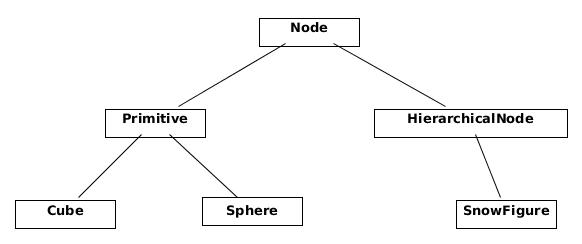
\includegraphics{nodes.jpg?raw=true}
\caption{The hierarchy of \texttt{Node} subclasses.}
\end{figure}

\begin{verbatim}
class HierarchicalNode(Node):
    def __init__(self):
        super(HierarchicalNode, self).__init__()
        self.child_nodes = []

    def render_self(self):
        for child in self.child_nodes:
            child.render()


class SnowFigure(HierarchicalNode):
    def __init__(self):
        super(SnowFigure, self).__init__()
        self.child_nodes = [Sphere(), Sphere(), Sphere()]
        self.child_nodes[0].translate(0, -0.6, 0) # scale 1.0
        self.child_nodes[1].translate(0, 0.1, 0)
        self.child_nodes[1].scaling_matrix = numpy.dot(
            self.scaling_matrix, scaling([0.8, 0.8, 0.8]))
        self.child_nodes[2].translate(0, 0.75, 0)
        self.child_nodes[2].scaling_matrix = numpy.dot(
            self.scaling_matrix, scaling([0.7, 0.7, 0.7]))
        for child_node in self.child_nodes:
            child_node.color_index = color.MIN_COLOR
        self.aabb = AABB([0.0, 0.0, 0.0], [0.5, 1.1, 0.5])
\end{verbatim}

You might observe that the \texttt{Node} objects form a tree data
structure. The \texttt{render} function, through hierarchical nodes,
does a depth-first traversal through the tree. As it traverses, it keeps
a stack of \texttt{ModelView} matrices, used for conversion into the
world space. At each step, it pushes the current \texttt{ModelView}
matrix onto the stack, and when it completes rendering of all child
nodes, it pops the matrix off the stack, leaving the parent node's
\texttt{ModelView} matrix at the top of the stack.

By making the \texttt{Node} class extensible in this way, we can add new
types of shapes to the scene without changing any of the other code for
scene manipulation and rendering. Using the node concept to abstract
away the fact that one \texttt{Scene} object may have many children is
known as the Composite design pattern.

\aosasectii{User Interaction}\label{user-interaction}

Now that our modeller is capable of storing and displaying the scene, we
need a way to interact with it. There are two types of interactions that
we need to facilitate. First, we need the capability of changing the
viewing perspective of the scene. We want to be able to move the eye, or
camera, around the scene. Second, we need to be able to add new nodes
and to modify nodes in the scene.

To enable user interaction, we need to know when the user presses keys
or moves the mouse. Luckily, the operating system already knows when
these events happen. GLUT allows us to register a function to be called
whenever a certain event occurs. We write functions to interpret key
presses and mouse movement, and tell GLUT to call those functions when
the corresponding keys are pressed. Once we know which keys the user is
pressing, we need to interpret the input and apply the intended actions
to the scene.

The logic for listening to operating system events and interpreting
their meaning is found in the \texttt{Interaction} class. The
\texttt{Viewer} class we wrote earlier owns the single instance of
\texttt{Interaction}. We will use the GLUT callback mechanism to
register functions to be called when a mouse button is pressed
(\texttt{glutMouseFunc}), when the mouse is moved
(\texttt{glutMotionFunc}), when a keyboard button is pressed
(\texttt{glutKeyboardFunc}), and when the arrow keys are pressed
(\texttt{glutSpecialFunc}). We'll see the functions that handle input
events shortly.

\begin{verbatim}
class Interaction(object):
    def __init__(self):
        """ Handles user interaction """
        # currently pressed mouse button
        self.pressed = None
        # the current location of the camera
        self.translation = [0, 0, 0, 0]
        # the trackball to calculate rotation
        self.trackball = trackball.Trackball(theta = -25, distance=15)
        # the current mouse location
        self.mouse_loc = None
        # Unsophisticated callback mechanism
        self.callbacks = defaultdict(list)
        
        self.register()

    def register(self):
        """ register callbacks with glut """
        glutMouseFunc(self.handle_mouse_button)
        glutMotionFunc(self.handle_mouse_move)
        glutKeyboardFunc(self.handle_keystroke)
        glutSpecialFunc(self.handle_keystroke)
\end{verbatim}

\aosasectiii{Operating System
Callbacks}\label{operating-system-callbacks}

In order to meaningfully interpret user input, we need to combine
knowledge of the mouse position, mouse buttons, and keyboard. Because
interpreting user input into meaningful actions requires many lines of
code, we encapsulate it in a separate class, away from the main code
path. The \texttt{Interaction} class hides unrelated complexity from the
rest of the codebase and translates operating system events into
application-level events.

\begin{verbatim}
    # class Interaction 
    def translate(self, x, y, z):
        """ translate the camera """
        self.translation[0] += x
        self.translation[1] += y
        self.translation[2] += z

    def handle_mouse_button(self, button, mode, x, y):
        """ Called when the mouse button is pressed or released """
        xSize, ySize = glutGet(GLUT_WINDOW_WIDTH), glutGet(GLUT_WINDOW_HEIGHT)
        y = ySize - y  # invert the y coordinate because OpenGL is inverted
        self.mouse_loc = (x, y)

        if mode == GLUT_DOWN:
            self.pressed = button
            if button == GLUT_RIGHT_BUTTON:
                pass
            elif button == GLUT_LEFT_BUTTON:  # pick
                self.trigger('pick', x, y)
            elif button == 3:  # scroll up
                self.translate(0, 0, 1.0)
            elif button == 4:  # scroll up
                self.translate(0, 0, -1.0)
        else:  # mouse button release
            self.pressed = None
        glutPostRedisplay()

    def handle_mouse_move(self, x, screen_y):
        """ Called when the mouse is moved """
        xSize, ySize = glutGet(GLUT_WINDOW_WIDTH), glutGet(GLUT_WINDOW_HEIGHT)
        y = ySize - screen_y  # invert the y coordinate because OpenGL is inverted
        if self.pressed is not None:
            dx = x - self.mouse_loc[0]
            dy = y - self.mouse_loc[1]
            if self.pressed == GLUT_RIGHT_BUTTON and self.trackball is not None:
                # ignore the updated camera loc because we want to always
                # rotate around the origin
                self.trackball.drag_to(self.mouse_loc[0], self.mouse_loc[1], dx, dy)
            elif self.pressed == GLUT_LEFT_BUTTON:
                self.trigger('move', x, y)
            elif self.pressed == GLUT_MIDDLE_BUTTON:
                self.translate(dx/60.0, dy/60.0, 0)
            else:
                pass
            glutPostRedisplay()
        self.mouse_loc = (x, y)

    def handle_keystroke(self, key, x, screen_y):
        """ Called on keyboard input from the user """
        xSize, ySize = glutGet(GLUT_WINDOW_WIDTH), glutGet(GLUT_WINDOW_HEIGHT)
        y = ySize - screen_y
        if key == 's':
            self.trigger('place', 'sphere', x, y)
        elif key == 'c':
            self.trigger('place', 'cube', x, y)
        elif key == GLUT_KEY_UP:
            self.trigger('scale', up=True)
        elif key == GLUT_KEY_DOWN:
            self.trigger('scale', up=False)
        elif key == GLUT_KEY_LEFT:
            self.trigger('rotate_color', forward=True)
        elif key == GLUT_KEY_RIGHT:
            self.trigger('rotate_color', forward=False)
        glutPostRedisplay()
\end{verbatim}

\aosasectiii{Internal Callbacks}\label{internal-callbacks}

In the code snippet above, you will notice that when the
\texttt{Interaction} instance interprets a user action, it calls
\texttt{self.trigger} with a string describing the action type. The
\texttt{trigger} function on the \texttt{Interaction} class is part of a
simple callback system that we will use for handling application-level
events. Recall that the \texttt{init\_interaction} function on the
\texttt{Viewer} class registers callbacks on the \texttt{Interaction}
instance by calling \texttt{register\_callback}.

\begin{verbatim}
    # class Interaction
    def register_callback(self, name, func):
        self.callbacks[name].append(func)
\end{verbatim}

When user interface code needs to trigger an event on the scene, the
\texttt{Interaction} class calls all of the saved callbacks it has for
that specific event:

\begin{verbatim}
    # class Interaction
    def trigger(self, name, *args, **kwargs):
        for func in self.callbacks[name]:
            func(*args, **kwargs)
\end{verbatim}

This application-level callback system abstracts away the need for the
rest of the system to know about operating system input. Each
application-level callback represents a meaningful request within the
application. The \texttt{Interaction} class acts as a translator between
operating system events and application-level events. This means that if
we decided to port the modeller to another toolkit in addition to GLUT,
we would only need to replace the \texttt{Interaction} class with a
class that converts the input from the new toolkit into the same set of
meaningful application-level callbacks.

We use the following callbacks and arguments:

\begin{table}
\centering
{\footnotesize
\rowcolors{2}{TableOdd}{TableEven}
\begin{tabular}{lll}
\hline
\textbf{Callback}
& \textbf{Arguments}
& \textbf{Purpose}
\\
\hline
pick    
& x:number, y:number 
& Selects the node at the mouse pointer location
\\
place & 
shape:string, x:number, y:number & 
Places a shape of the specified type at the mouse pointer location.
\\
rotate\_color & 
forward:boolean & 
Rotates the color of the currently selected node.
\\
scale & 
up:boolean & 
Scales the currently selected node up or down.
\\
\hline
\end{tabular}
}
\caption{Interaction callbacks and arguments}
\label{500l.tbl.callbacks}
\end{table}

This simple callback system provides all of the functionality we need
for this project. In a production 3D modeller, however, user interface
objects are often created and destroyed dynamically. In that case, we
would need a more sophisticated event listening system, where objects
can both register and un-register callbacks for events.

\aosasectii{Interfacing with the
Scene}\label{interfacing-with-the-scene}

With our callback mechanism, we can receive meaningful information about
user input events from the \texttt{Interaction} class. We are ready to
apply these actions to the \texttt{Scene}.

\aosasectiii{Moving the Scene}\label{moving-the-scene}

In this project, we accomplish camera motion by transforming the scene.
In other words, the camera is at a fixed location and user input moves
the scene instead of moving the camera. The camera is placed at
\texttt{{[}0, 0, -15{]}} and faces the world space origin.
(Alternatively, we could change the perspective matrix to move the
camera instead of the scene. This design decision has very little impact
on the rest of the project.) Revisiting the \texttt{render} function in
the \texttt{Viewer}, we see that the \texttt{Interaction} state is used
to transform the OpenGL matrix state before rendering the
\texttt{Scene}. There are two types of interaction with the scene:
rotation and translation.

\aosasectiii{Rotating the Scene with a
Trackball}\label{rotating-the-scene-with-a-trackball}

We accomplish rotation of the scene by using a \emph{trackball}
algorithm. The trackball is an intuitive interface for manipulating the
scene in three dimensions. Conceptually, a trackball interface functions
as if the scene was inside a transparent globe. Placing a hand on the
surface of the globe and pushing it rotates the globe. Similarly,
clicking the right mouse button and moving it on the screen rotates the
scene. You can find out more about the theory of the trackball at the
\href{http://www.opengl.org/wiki/Object_Mouse_Trackball}{OpenGL Wiki}.
In this project, we use a trackball implementation provided as part of
\href{https://code.google.com/p/glumpy/source/browse/glumpy/trackball.py}{Glumpy}.

We interact with the trackball using the \texttt{drag\_to} function,
with the current location of the mouse as the starting location and the
change in mouse location as parameters.

\begin{verbatim}
self.trackball.drag_to(self.mouse_loc[0], self.mouse_loc[1], dx, dy)
\end{verbatim}

The resulting rotation matrix is retrieved as \texttt{trackball.matrix}
in the viewer when the scene is rendered.

\aosasectiii{Aside: Quaternions}\label{aside-quaternions}

Rotations are traditionally represented in one of two ways. The first is
a rotation value around each axis; you could store this as a 3-tuple of
floating point numbers. The other common representation for rotations is
a quaternion, an element composed of a vector with $x$, $y$, and $z$
coordinates, and a $w$ rotation. Using quaternions has numerous benefits
over per-axis rotation; in particular, they are more numerically stable.
Using quaternions avoids problems like gimbal lock. The downside of
quaternions is that they are less intuitive to work with and harder to
understand. If you are brave and would like to learn more about
quaternions, you can refer to \href{http://3dgep.com/?p=1815}{this
explanation}.

The trackball implementation avoids gimbal lock by using quaternions
internally to store the rotation of the scene. Luckily, we do not need
to work with quaternions directly, because the matrix member on the
trackball converts the rotation to a matrix.

\aosasectiii{Translating the Scene}\label{translating-the-scene}

Translating the scene (i.e., sliding it) is much simpler than rotating
it. Scene translations are provided with the mouse wheel and the left
mouse button. The left mouse button translates the scene in the $x$ and
$y$ coordinates. Scrolling the mouse wheel translates the scene in the z
coordinate (towards or away from the camera). The \texttt{Interaction}
class stores the current scene translation and modifies it with the
\texttt{translate} function. The viewer retrieves the
\texttt{Interaction} camera location during rendering to use in a
\texttt{glTranslated} call.

\aosasectiii{Selecting Scene Objects}\label{selecting-scene-objects}

Now that the user can move and rotate the entire scene to get the
perspective they want, the next step is to allow the user to modify and
manipulate the objects that make up the scene.

In order for the user to manipulate objects in the scene, they need to
be able to select items.

To select an item, we use the current projection matrix to generate a
ray that represents the mouse click, as if the mouse pointer shoots a
ray into the scene. The selected node is the closest node to the camera
with which the ray intersects. Thus the problem of picking reduced to
the problem of finding intersections between a ray and nodes in the
scene. So the question is: How do we tell if the ray hits a node?

Calculating exactly whether a ray intersects with a node is a
challenging problem in terms of both complexity of code and of
performance. We would need to write a ray-object intersection check for
each type of primitive. For scene nodes with complex mesh geometries
with many faces, calculating exact ray-object intersection would require
testing the ray against each face and would be computationally
expensive.

For the purposes of keeping the code compact and performance reasonable,
we use a simple, fast approximation for the ray-object intersection
test. In our implementation, each node stores an axis-aligned bounding
box (AABB), which is an approximation of the space it occupies. To test
whether a ray intersects with a node, we test whether the ray intersects
with the node's AABB. This implementation means that all nodes share the
same code for intersection tests, and it means that the performance cost
is constant and small for all node types.

\begin{verbatim}
    # class Viewer
    def get_ray(self, x, y):
        """ 
        Generate a ray beginning at the near plane, in the direction that
        the x, y coordinates are facing 

        Consumes: x, y coordinates of mouse on screen 
        Return: start, direction of the ray 
        """
        self.init_view()
    
        glMatrixMode(GL_MODELVIEW)
        glLoadIdentity()
    
        # get two points on the line.
        start = numpy.array(gluUnProject(x, y, 0.001))
        end = numpy.array(gluUnProject(x, y, 0.999))
    
        # convert those points into a ray
        direction = end - start
        direction = direction / norm(direction)
    
        return (start, direction)
    
    def pick(self, x, y):
        """ Execute pick of an object. Selects an object in the scene. """
        start, direction = self.get_ray(x, y)
        self.scene.pick(start, direction, self.modelView)
\end{verbatim}

To determine which node was clicked on, we traverse the scene to test
whether the ray hits any nodes. We deselect the currently selected node
and then choose the node with the intersection closest to the ray
origin.

\begin{verbatim}
    # class Scene
    def pick(self, start, direction, mat):
        """ 
        Execute selection.
            
        start, direction describe a Ray. 
        mat is the inverse of the current modelview matrix for the scene.
        """
        if self.selected_node is not None:
            self.selected_node.select(False)
            self.selected_node = None
    
        # Keep track of the closest hit.
        mindist = sys.maxint
        closest_node = None
        for node in self.node_list:
            hit, distance = node.pick(start, direction, mat)
            if hit and distance < mindist:
                mindist, closest_node = distance, node
    
        # If we hit something, keep track of it.
        if closest_node is not None:
            closest_node.select()
            closest_node.depth = mindist
            closest_node.selected_loc = start + direction * mindist
            self.selected_node = closest_node
\end{verbatim}

Within the \texttt{Node} class, the \texttt{pick} function tests whether
the ray intersects with the axis-aligned bounding box of the
\texttt{Node}. If a node is selected, the \texttt{select} function
toggles the selected state of the node. Notice that the AABB's
\texttt{ray\_hit} function accepts the transformation matrix between the
box's coordinate space and the ray's coordinate space as the third
parameter. Each node applies its own transformation to the matrix before
making the \texttt{ray\_hit} function call.

\begin{verbatim}
    # class Node
    def pick(self, start, direction, mat):
        """ 
        Return whether or not the ray hits the object

        Consume:  
        start, direction form the ray to check
        mat is the modelview matrix to transform the ray by 
        """

        # transform the modelview matrix by the current translation
        newmat = numpy.dot(
            numpy.dot(mat, self.translation_matrix), 
            numpy.linalg.inv(self.scaling_matrix)
        )
        results = self.aabb.ray_hit(start, direction, newmat)
        return results

    def select(self, select=None):
       """ Toggles or sets selected state """
       if select is not None:
           self.selected = select
       else:
           self.selected = not self.selected
    
\end{verbatim}

The ray-AABB selection approach is very simple to understand and
implement. However, the results are wrong in certain situations.

\aosafigure[240pt]{modeller-images/AABBError.png}{AABB Error}{500l.modeller.aabberror}

For example, in the case of the \texttt{Sphere} primitive, the sphere
itself only touches the AABB in the centre of each of the AABB's faces.
However if the user clicks on the corner of the Sphere's AABB, the
collision will be detected with the Sphere, even if the user intended to
click past the Sphere onto something behind it
(\aosafigref{500l.modeller.aabberror}).

This trade-off between complexity, performance, and accuracy is common
in computer graphics and in many areas of software engineering.

\aosasectiii{Modifying Scene Objects}\label{modifying-scene-objects}

Next, we would like to allow the user to manipulate the selected nodes.
They might want to move, resize, or change the color of the selected
node. When the user inputs a command to manipulate a node, the
\texttt{Interaction} class converts the input into the action that the
user intended, and calls the corresponding callback.

When the \texttt{Viewer} receives a callback for one of these events, it
calls the appropriate function on the \texttt{Scene}, which in turn
applies the transformation to the currently selected \texttt{Node}.

\begin{verbatim}
    # class Viewer
    def move(self, x, y):
        """ Execute a move command on the scene. """
        start, direction = self.get_ray(x, y)
        self.scene.move_selected(start, direction, self.inverseModelView)
    
    def rotate_color(self, forward):
        """ 
        Rotate the color of the selected Node. 
        Boolean 'forward' indicates direction of rotation. 
        """
        self.scene.rotate_selected_color(forward)
    
    def scale(self, up):
        """ Scale the selected Node. Boolean up indicates scaling larger."""
        self.scene.scale_selected(up)
\end{verbatim}

\aosasectiii{Changing Color}\label{changing-color}

Manipulating color is accomplished with a list of possible colors. The
user can cycle through the list with the arrow keys. The scene
dispatches the color change command to the currently selected node.

\begin{verbatim}
    # class Scene
    def rotate_selected_color(self, forwards):
        """ Rotate the color of the currently selected node """
        if self.selected_node is None: return
        self.selected_node.rotate_color(forwards)
\end{verbatim}

Each node stores its current color. The \texttt{rotate\_color} function
simply modifies the current color of the node. The color is passed to
OpenGL with \texttt{glColor} when the node is rendered.

\begin{verbatim}
    # class Node
    def rotate_color(self, forwards):
        self.color_index += 1 if forwards else -1
        if self.color_index > color.MAX_COLOR:
            self.color_index = color.MIN_COLOR
        if self.color_index < color.MIN_COLOR:
            self.color_index = color.MAX_COLOR
\end{verbatim}

\aosasectiii{Scaling Nodes}\label{scaling-nodes}

As with color, the scene dispatches any scaling modifications to the
selected node, if there is one.

\begin{verbatim}
    # class Scene
    def scale_selected(self, up):
        """ Scale the current selection """
        if self.selected_node is None: return
        self.selected_node.scale(up)
    
\end{verbatim}

Each node stores a current matrix that stores its scale. A matrix that
scales by parameters $x$, $y$ and $z$ in those respective directions is:

\[
   \begin{bmatrix}
   x & 0 & 0 & 0 \\
   0 & y & 0 & 0 \\
   0 & 0 & z & 0 \\
   0 & 0 & 0 & 1 \\
   \end{bmatrix}
\]

When the user modifies the scale of a node, the resulting scaling matrix
is multiplied into the current scaling matrix for the node.

\begin{verbatim}
    # class Node
    def scale(self, up):
        s =  1.1 if up else 0.9
        self.scaling_matrix = numpy.dot(self.scaling_matrix, scaling([s, s, s]))
        self.aabb.scale(s)
\end{verbatim}

The function \texttt{scaling} returns such a matrix, given a list
representing the $x$, $y$, and $z$ scaling factors.

\begin{verbatim}
def scaling(scale):
    s = numpy.identity(4)
    s[0, 0] = scale[0]
    s[1, 1] = scale[1]
    s[2, 2] = scale[2]
    s[3, 3] = 1
    return s
\end{verbatim}

\aosasectiii{Moving Nodes}\label{moving-nodes}

In order to translate a node, we use the same ray calculation we used
for picking. We pass the ray that represents the current mouse location
in to the scene's \texttt{move} function. The new location of the node
should be on the ray. In order to determine where on the ray to place
the node, we need to know the node's distance from the camera. Since we
stored the node's location and distance from the camera when it was
selected (in the \texttt{pick} function), we can use that data here. We
find the point that is the same distance from the camera along the
target ray and we calculate the vector difference between the new and
old locations. We then translate the node by the resulting vector.

\begin{verbatim}
    # class Scene
    def move_selected(self, start, direction, inv_modelview):
        """ 
        Move the selected node, if there is one.
            
        Consume: 
        start, direction describes the Ray to move to
        mat is the modelview matrix for the scene 
        """
        if self.selected_node is None: return
    
        # Find the current depth and location of the selected node
        node = self.selected_node
        depth = node.depth
        oldloc = node.selected_loc
    
        # The new location of the node is the same depth along the new ray
        newloc = (start + direction * depth)
    
        # transform the translation with the modelview matrix
        translation = newloc - oldloc
        pre_tran = numpy.array([translation[0], translation[1], translation[2], 0])
        translation = inv_modelview.dot(pre_tran)
    
        # translate the node and track its location
        node.translate(translation[0], translation[1], translation[2])
        node.selected_loc = newloc
\end{verbatim}

Notice that the new and old locations are defined in the camera
coordinate space. We need our translation to be defined in the world
coordinate space. Thus, we convert the camera space translation into a
world space translation by multiplying by the inverse of the modelview
matrix.

As with scale, each node stores a matrix which represents its
translation. A translation matrix looks like:

\[
   \begin{bmatrix}
   1 & 0 & 0 & x \\
   0 & 1 & 0 & y \\
   0 & 0 & 1 & z \\
   0 & 0 & 0 & 1 \\
   \end{bmatrix}
\]

When the node is translated, we construct a new translation matrix for
the current translation, and multiply it into the node's translation
matrix for use during rendering.

\begin{verbatim}
    # class Node
    def translate(self, x, y, z):
        self.translation_matrix = numpy.dot(self.translation_matrix, translation([x, y, z]))
\end{verbatim}

The \texttt{translation} function returns a translation matrix given a
list representing the $x$, $y$, and $z$ translation distances.

\begin{verbatim}
def translation(displacement):
    t = numpy.identity(4)
    t[0, 3] = displacement[0]
    t[1, 3] = displacement[1]
    t[2, 3] = displacement[2]
    return t
\end{verbatim}

\aosasectiii{Placing Nodes}\label{placing-nodes}

Node placement uses techniques from both picking and translation. We use
the same ray calculation for the current mouse location to determine
where to place the node.

\begin{verbatim}
    # class Viewer
    def place(self, shape, x, y):
        """ Execute a placement of a new primitive into the scene. """
        start, direction = self.get_ray(x, y)
        self.scene.place(shape, start, direction, self.inverseModelView)
\end{verbatim}

To place a new node, we first create the new instance of the
corresponding type of node and add it to the scene. We want to place the
node underneath the user's cursor, so we find a point on the ray, at a
fixed distance from the camera. Again, the ray is represented in camera
space, so we convert the resulting translation vector into the world
coordinate space by multiplying it by the inverse modelview matrix.
Finally, we translate the new node by the calculated vector.

\begin{verbatim}
    # class Scene
    def place(self, shape, start, direction, inv_modelview):
        """ 
        Place a new node.
            
        Consume:  
        shape the shape to add
        start, direction describes the Ray to move to
        inv_modelview is the inverse modelview matrix for the scene 
        """
        new_node = None
        if shape == 'sphere': new_node = Sphere()
        elif shape == 'cube': new_node = Cube()
        elif shape == 'figure': new_node = SnowFigure()
    
        self.add_node(new_node)
    
        # place the node at the cursor in camera-space
        translation = (start + direction * self.PLACE_DEPTH)
    
        # convert the translation to world-space
        pre_tran = numpy.array([translation[0], translation[1], translation[2], 1])
        translation = inv_modelview.dot(pre_tran)
    
        new_node.translate(translation[0], translation[1], translation[2])
\end{verbatim}

\aosasecti{Summary}\label{summary}

Congratulations! We've successfully implemented a tiny 3D modeller!

\aosafigure[240pt]{modeller-images/StartScene.png}{Sample Scene}{500l.modeller.samplescene}

We saw how to develop an extensible data structure to represent the
objects in the scene. We noticed that using the Composite design pattern
and a tree-based data structure makes it easy to traverse the scene for
rendering and allows us to add new types of nodes with no added
complexity. We leveraged this data structure to render the design to the
screen, and manipulated OpenGL matrices in the traversal of the scene
graph. We built a very simple callback system for application-level
events, and used it to encapsulate handling of operating system events.
We discussed possible implementations for ray-object collision
detection, and the trade-offs between correctness, complexity, and
performance. Finally, we implemented methods for manipulating the
contents of the scene.

You can expect to find these same basic building blocks in production 3D
software. The scene graph structure and relative coordinate spaces are
found in many types of 3D graphics applications, from CAD tools to game
engines. One major simplification in this project is in the user
interface. A production 3D modeller would be expected to have a complete
user interface, which would necessitate a much more sophisticated events
system instead of our simple callback system.

We could do further experimentation to add new features to this project.
Try one of these:

\begin{aosaitemize}

\item
  Add a \texttt{Node} type to support triangle meshes for arbitrary
  shapes.
\item
  Add an undo stack, to allow undo/redo of modeller actions.
\item
  Save/load the design using a 3D file format like DXF.
\item
  Integrate a rendering engine: export the design for use in a
  photorealistic renderer.
\item
  Improve collision detection with accurate ray-object intersection.
\end{aosaitemize}

\aosasecti{Further Exploration}\label{further-exploration}

For further insight into real-world 3D modelling software, a few open
source projects are interesting.

\href{http://www.blender.org/}{Blender} is an open source full-featured
3D animation suite. It provides a full 3D pipeline for building special
effects in video, or for game creation. The modeller is a small part of
this project, and it is a good example of integrating a modeller into a
large software suite.

\href{http://www.openscad.org/}{OpenSCAD} is an open source 3D modelling
tool. It is not interactive; rather, it reads a script file that
specifies how to generate the scene. This gives the designer ``full
control over the modelling process''.

For more information about algorithms and techniques in computer
graphics, \href{http://tog.acm.org/resources/GraphicsGems/}{Graphics
Gems} is a great resource.

\end{aosachapter}
